\tikzstyle{arrow} = [thick,->,>=stealth]
\tikzstyle{subject} = [ circle, minimum size=2cm, draw=black ]
\tikzstyle{resource} = [rectangle, minimum height=2cm,  minimum width=2.5cm, draw=black, anchor=east, font=\ttfamily,]
\tikzstyle{clist} = [draw, rectangle, rounded corners=20pt, minimum height=2.5cm]
\tikzstyle{capability} = [draw, inner sep=1mm, anchor=west, minimum width=1cm, font=\ttfamily,]
\tikzstyle{mymatrix} = [matrix of nodes, nodes=capability, row sep=1mm]

        \begin{subfigure}[b]{0.49\textwidth}
    \centering
    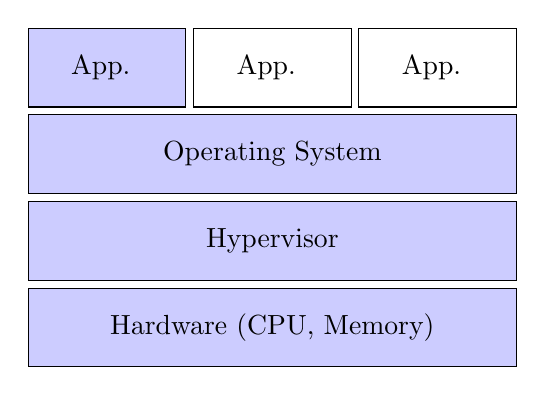
\begin{tikzpicture}[node distance=1.1cm]
\node (hw) [rectangle, draw,align=center, minimum width=6.2cm, minimum height=1cm,fill=blue!20] {Hardware (CPU, Memory)};

\node (hyp) [rectangle,draw,align=center,above of=hw, minimum width=6.2cm, minimum height=1cm,fill=blue!20] {Hypervisor};
\node (os) [rectangle,draw,align=center,above of=hyp, minimum width=6.2cm, minimum height=1cm, fill=blue!20] {Operating System};

\node (app1) [rectangle,draw,align=left,above of=os, minimum width=2cm, minimum height=1cm, xshift=-2.1cm, fill=blue!20] {App. };
\node (app2) [rectangle,draw,align=left,right of=app1, minimum width=2cm, minimum height=1cm, xshift=1cm] {App. };
\node (app3) [rectangle,draw,align=left,right of=app2, minimum width=2cm, minimum height=1cm, xshift=1cm] {App. };

% \node (legend1) [rectangle, draw, fill=blue!20, right of=hw, xshift=3cm]{}; 
% \node (legend2) [rectangle, draw, yshift=-0.5cm, above of=legend1]{}; 
% \node (cap1) [right of=legend1, align=left]{Untrusted};
% \node (cap2) [right of=legend2, align=left]{Trusted};

\end{tikzpicture}
    \caption{Trust model of traditional computing.}
    \label{fig:bg:acl}
    \end{subfigure}
        \begin{subfigure}[b]{0.49\textwidth}
    \centering
    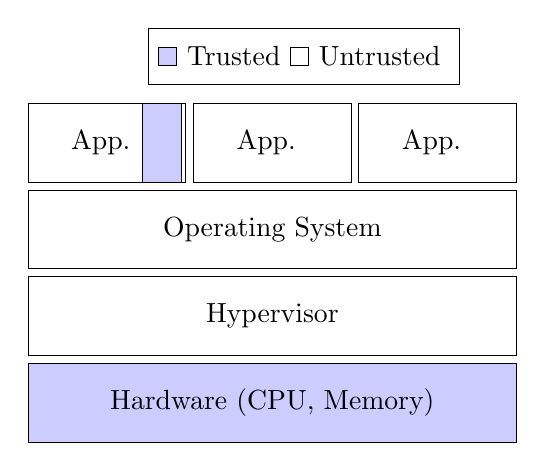
\begin{tikzpicture}[node distance=1.1cm]
\node (hw) [rectangle, draw,align=center, minimum width=6.2cm, minimum height=1cm,fill=blue!20] {Hardware (CPU, Memory)};

\node (hyp) [rectangle,draw,align=center,above of=hw, minimum width=6.2cm, minimum height=1cm] {Hypervisor};
\node (os) [rectangle,draw,align=center,above of=hyp, minimum width=6.2cm, minimum height=1cm] {Operating System};

\node (app1) [rectangle,draw,align=left,above of=os, minimum width=2cm, minimum height=1cm, xshift=-2.1cm] {App. };
\node (app1t) [rectangle,draw,align=left,above of=os, minimum width=0.5cm, minimum height=1cm, xshift=-1.4cm,fill=blue!20] {};
\node (app2) [rectangle,draw,align=left,right of=app1, minimum width=2cm, minimum height=1cm, xshift=1cm] {App. };
\node (app3) [rectangle,draw,align=left,right of=app2, minimum width=2cm, minimum height=1cm, xshift=1cm] {App. };

% Legend
\matrix [draw, above of =app1, xshift=2.5cm] {
  \node [rectangle,draw,fill=blue!20,label=right:Trusted] {};&  \node [rectangle,draw,label=right:Untrusted] {}; \\
};

\end{tikzpicture}
    \caption{Trust model of Process-based TEEs.}
    \label{fig:bg:trust-model-tee}
    \end{subfigure}

